\documentclass[12pt,a4paper]{article} % document setting, articles do not allow chapters
\usepackage[english]{babel} % english spell-check
\usepackage[utf8]{inputenc} % allows the input of special characters from keyboard
\usepackage[T1]{fontenc}
\usepackage{lmodern} %load modern fonts
\usepackage{helvet} % lead helvetica font
\renewcommand{\familydefault}{\sfdefault} % without this helvetica does not work on linux
\usepackage{textcomp} % for text symbols such as (C)
\usepackage{siunitx} % for mathematical embedding with $

\AtBeginDocument{\renewcommand{\bibname}{References}} % change Bibliography to Reference in TOC
%\usepackage[super, numbers]{natbib} % include bibliography
%\bibliographystyle{unsrtnat} % order by appearance
\usepackage[compress]{natbib}
\bibliographystyle{apalike} % simple bibliography style % sudo texhash
%\bibliographystyle{plainnat}
\usepackage{hyperref} % allow printing URLs (here: for Bibliography)
\usepackage{cite}

\usepackage{graphicx} % include figures
\usepackage[labelfont=bf]{caption} % change figure caption to bold

\usepackage{titlesec} %change title style
\titleformat*{\section}{\normalsize\bfseries}
\titleformat*{\subsection}{\normalsize\itshape}

%\usepackage[mathlines]{lineno} % add line numbers
\usepackage{setspace} %for double spacing

\usepackage{booktabs}
\usepackage{makecell}

\author{Masumi Stadler}
\title{PhD Manuscript 1}

%%%%%%%%%%%%
% Document %
%%%%%%%%%%%%
\begin{document}
%\linenumbers

\setlength{\parindent}{0cm}
Title (max 150 char): Reactive bacterioplankton reveal assembly dynamics along a boreal terrestrial-aquatic continuum\\

Masumi Stadler\textsuperscript{1,*}, Paul A. del Giorgio\textsuperscript{1}\\

Affilitation:\\
(1) Groupe de Recherche Interuniversitaire en Limnologie (GRIL), D\'{e}partement des Sciences Biologiques, Universit\'{e} du Qu\'{e}bec \`{a} Montr\'{e}al, Montr\'{e}al, QC, Canada


Institutional e-mail addresses: MS (stadler.masumi@courrier.uqam.ca), PdG (del\_giorgio.paul@uqam.ca)\\

Running title (max 50 char): Bacterioplankton along a boreal terrestrial-hydrological continuum.\\

*Contact corresponding author: Masumi Stadler \\
E-mail: m.stadler.jp.at@gmail.com \\
Phone: +1 (514)297-5330 \\
Address: D\'{e}partement des Sciences Biologiques, Universit\'{e} du Qu\'{e}bec \`{a} Montr\'{e}al, Case Postale 8888, Succursale Centre-Ville, Montr\'{e}al, QC, H3C 3P8, Canada \\

Keywords: aquatic bacterial communities, bacterioplankton, terrestrial-aquatic continuum, ecosystem connectivity, boreal ecosystems, mass effects, environmental sorting, metacommunity, meta-ecosystem, coalescence, microbial assembly, rare biosphere, rank abundance\\

Author contributions: PdG designed the sampling, MS collected the data, MS analysed the data, MS and PdG discussed the results and wrote the manuscript.\\

\newpage

\doublespacing

\section*{Abstract} % 200 words
%\begin{abstract}
Inland waters form complex hydrological networks acting as a bridge of abiotic and biotic matter between the terrestrial milieu and ultimately the oceans. During transport through the aquatic network, microbial communities are modified and re-assembled, forming complex patterns of ecological successions. These processes have seldom been examined along a true land-estuary aquatic continuum. Here we reconstruct the microbial succession from soils through the aquatic network until the estuary within the Romaine River watershed in Eastern Québec over three years. Two discontinuities along the river (riverine lakes and reservoirs) create a unique opportunity to address shifts in residence times within an assembly context. In order to distinguish the total from the reactive fraction of microbial communities we sequenced the 16S rRNA amplicon DNA and RNA. Differences among microbial assemblages was mainly driven by habitat type and seasons. Different patterns in incidence and abundance based DNA and RNA dissimilarity revealed dominating mass effects whenever two contrasting communities mix, such as terrestrial-aquatic as well as reservoir hypolimnetic-riverine transitions. In general, increasing residence time favoured stronger selection over mass effects. Our findings highlight the importance of considering spatial history and distinguishing the total and active microbial fractions, especially in highly connected and dynamic systems.
%\end{abstract}


% main text 5000 words (excluding abstract, tables/figures, and references)
\setlength{\parindent}{1cm}
\section*{Introduction}
Microbial communities across ecosystems are characterized by rank abundance distributions that vary in shape, yet, we still know relatively little on how these structures come to be. Distribution shapes are thought to provide insight on community assembly \citep{McGill2007}, with dominant and rare taxa assumed to be locally successful and transient, respectively \citep{Magurran2003, Nakadai2020}, but, these interpretations have seldom been explicitly confirmed. Inherited from macro-ecology, microbial assembly processes have been defined into four fundamental categories - selection, dispersal, diversification and drift - \citep{Vellend2010}, which vary in their degree of determinism and stochasticity \citep{Zhou2017}. Whereas diversification and drift usually manifest on longer, evolutionary, time scales, selection as well as dispersal are more relevant on ecological time scales. Regardless, there is always a historical aspect to community assembly as local microbial communities reflect the balance between selection and dispersal processes that have occurred locally and in connected habitats in the past \citep{Fukami2004}. Hence, accounting for community history is vital to understand community assembly and the shape of the rank abundance distribution.

Studies that investigated the relevance of history mainly followed microbes in time within an ecosystem \citep{Shade2015b}. Temporal history does shape local communities (i.e. legacy effects, \citet{Fukami2015a}), however, within an aquatic network, the uni-directional flow of water links temporal to spatial history. Hydrology is a major driver of aquatic microbial community composition \citep{Nino-Garcia2016}, as evidenced by soil microbes being flushed into and representing large proportions of aquatic communities \citep{Ruiz-Gonzalez2015, Hauptmann2016, Crump2012, Besemer2013, Wisnoski2020}. As such, community structure at any given site within a fluvial network is the net result of upstream assembly processes, and network connectivity is further modulated by seasonal hydrological fluctuations \citep{deMelo2019, Caillon2021}. Therefore, spatial history is particularly relevant in highly interconnected freshwater networks \citep{Vass2017}, and there have been various studies that investigated the spatial context of aquatic microbial community assembly. \citet{Stegen2013a} quantified major assembly processes based on spatial patterns of phylogenetic as well as taxonomic dispersion, which assumes that phylogenetically related organisms have similar niche requirements. Others have used spatial numerical distributions to infer the relative importance of selection versus passive transport across separate watersheds \citep{Nino-Garcia2016b}. While the importance of mingling and interacting communities between different ecosystems is now amply recognized (i.e. community coalescence, \citet{Mansour2018}), few studies consider interfaces between multiple ecosystems or ecosystem domains (e.g. terrestrial - aquatic) \citep{Nemergut2011, Shade2013}. A spatially connected, true aquatic continuum has mostly been evaluated on local scales of lakes \citep{Logue2010, Adams2014, Langenheder2017}, along a single river \citep{Winter2007, Savio2015a, Hauptmann2016, Doherty2017, Gweon2020} or on interconnected upstream networks \citep{Besemer2013, Widder2014, Read2015, Hassell2018, Wisnoski2020a} and rarely have surrounding terrestrial ecosystems been considered as potential sources \citep{Crump2012, Ruiz-Gonzalez2015, Wisnoski2020}. Moreover, active and passive assembly processes are difficult to resolve as cell death and dormancy blur interpretations based on DNA \citep{Cole1999, Jones2010}. Indicative of recent protein synthesis, RNA sequencing has helped to disentangle active from passive microbial members \citep{Bowsher2019}, however, only few freshwater studies have included both \citep{Logue2010, Szekely2013, Aanderud2016, Peter2018, Wisnoski2020}. All of these studies have separately yielded useful insight on microbial community assembly in freshwater systems, and they collectively point to the challenges ahead.

The processes shaping community assembly are dynamic; selection and mass effects will vary in relative importance along complex aquatic networks as a function of the degree of connectivity to surrounding ecosystems, and upstream history. In order to capture the shifting balance of assembly processes and link those to the underlying rank abundance structure, we firstly need to examine a true hydrologic continuum that includes source communities and exchanges between various aquatic as well as terrestrial habitats as potential sources. Secondly, seasonality needs to be accounted for as the degree of connectivity depends largely on various hydrological scenarios in these networks. And lastly, DNA has to be accompanied by some indication of reactivity as selection and passive dispersal cannot be fully distinguished otherwise. In this study, we attempted a more holistic approach to aquatic microbial community assembly by addressing the three aforementioned critical dimensions.

%To address these three points, we have sampled the Romaine river watershed in North-Eastern Québec, Canada, as an example boreal watershed over several years and seasons. The Romaine watershed is particularly interesting as it drains a large and heterogeneous watershed (Area: 14 500 km2), and it contains three reservoirs that have been consecutively flooded over the sampled years. The mid-river shift in residence time (RT) from riverine to lentic conditions and back to lotic conditions downstream of the reservoir complex allows us to assess how the processes underlying community assembly shift as communities experience these different environmental and hydrologic scenarios. Similarly, there is a chain of shallow lakes close to the Northern most headwater sub-catchment (hereafter riverine lakes), that additionally allows to study the effect of changing residence times on community structure in a more natural context. Stretching over 475 km, we captured much of the extant river order (from 0 to 7) and various interfaces (terrestrial-aquatic, freshwater-estuary, low RT-high RT), as well as ecosystems in the extended meta-community (e.g. headwater ponds, tributaries, lakes).

\subsection*{Conceptual framework}
Our overall aim was to follow shifts in bacterial community structure along a terrestrial aquatic continuum and assess how the relative importance of mass effects versus species selection changes as communities traverse through varying environmental conditions and degrees of connectivity to the surrounding catchment. We have carried out this study within La Romaine river watershed in the North-Eastern region of boreal Québec, Canada, over several years and seasons. Starting from upstream sources such as soils, soil-waters, and headwater streams, we continued to follow the extant river orders (Strahler order 0-8) up to the estuarine plume. Additionally, three reservoirs have been consecutively flooded mid-river over the sampling period. The sampling design covers various interfaces (terrestrial-aquatic, stream-river, river-reservoir, freshwater-estuary), and other ecosystems within the watershed (e.g. headwater ponds, tributaries, lakes) that provide a further meta-community context.

We first assess how the 16S rRNA gene (DNA-based) community structure shifts along the terrestrial-freshwater-estuary continuum; we determine the general patterns of the spatial succession and its relation to different hydrologic conditions (i.e. seasons). We further differentiate the reactive from the total bacterial assemblage by additionally sequencing RNA. We do not use RNA as an indication of activity per se (Blazewicz et al., 2013), rather we interpret the patterns of divergence and convergence of DNA-/RNA-based assemblage structures along the continuum to infer shifts in the relative importance of species selection versus mass effects. To quantify divergence between DNA-/RNA-based community structures, we developed distance metrics with either incidence (presence-absence) or abundance-based dissimilarities. In a null scenario, DNA-/RNA-based assemblage structure remains equidistant, which would indicate no influx of unreactive bacteria (i.e. only detectable in DNA), and no changes in the reactivity of taxa within the community (no inactivation and activation of active and dormant taxa, respectively). Local divergence in DNA-/RNA-based assemblage structures in the continuum, on the other hand, may result from an influx of bacteria unreactive to local conditions (low RNA detectability), which would strongly influence the incidence-based distance, or from local shifts in the reactivity of specific taxa within the community (reactive taxa), influencing mostly the abundance-based distance. The spatial patterns in the incidence- and abundance-based metrics therefore provide insight on how selection and mass effects vary along the continuum. Finally, we explore where taxa originate along the continuum and what fraction within the rank abundance curve the unreactive and reactive taxa commonly occupy.

% Similarly, there is a chain of shallow lakes close to the Northern most headwater sub-catchment (hereafter riverine lakes), that additionally allows to study the effect of changing residence times on community structure in a more natural context.
%Our overall aim was to follow a true aquatic continuum, capture the dominant sources and various ecosystems within a hydrological network and evaluate the relative importance of mass effect versus selection as communities encounter various changing environmental and hydrologic conditions. To differentiate between the total and reactive bacterial assemblages, we have sequenced the 16S rRNA gene (DNA) as well as its RNA, respectively. We do not use RNA as an indication of activity per se (Blazewicz et al., 2013), rather patterns of divergence and convergence of DNA- and RNA-based assemblage structures are utilized to infer shifts in the relative importance of species selection versus mass effects between different habitats along the continuum. To quantify relative DNA and RNA con- and divergence, we utilized multivariate distance metrics with either incidence (presence-absence) or abundance based dissimilarities. If the DNA- and RNA-based assemblage structure would be equidistant along the continuum, we would interpret such patterns as indicating no influx of passive, inactive bacteria, and no changes in the reactivity of all community members. Divergence in DNA and RNA assemblage structure, on the other hand, may result from an influx of inactive bacteria, which would influence strongly the incident based distance, or from shifts in the reactivity of selected taxa within the community, which would influence mostly the abundance based distance.
%In summary, we firstly determine the spatial restructuring of communities and its seasonality that occurs from headwater soils, streams to the main stem of the Romaine river onto the reservoirs, followed by a downstream river stretch until the estuary. We then superimpose RNA-based assemblage structures to further resolve the relative shifts in selection versus mass effects. And finally, we explore where within a typical RAD, DNA and RNA divergence is most prominent.

\section*{Material and methods}
\subsection*{Catchment characteristics and sampling}
To follow the movement of microbial communities within a watershed, samples were taken along La Romaine river (C\^{o}te-Nord region, Qu\'{e}bec, Canada) (Fig. 1a-b) for three years from 2015-2017. La Romaine catchment belongs to the eastern black spruce-moss bioclimatic domain and has an area (\textit{A}) of approximately 14 500 km\textsuperscript{2}. For detailed catchment characteristics refer to the supplementary methods (hereafter, SM) (SM1). In brief, the mainstem of the river flows through a series of large, shallow lakes (hereafter, riverine lakes), emerging as Strahler order 7, and is subsequently dammed in a series of three hydroelectric reservoirs that were consecutively built in 2015 (RO2), 2016 (RO1), and 2017 (RO3). We refer to the river sections before and after the reservoir complex as upriver and downriver, respectively. The river has a total distance from the northern headwaters to the river mouth expanding of approximately 475 km.

In order to follow a terrestrial-aquatic continuum, various habitat types were sampled (Table S1). To capture a headwater network with soils, soilwaters, streams and ponds, we sampled the Petite Romaine sub-catchment (PR, \textit{A}: 310.73 km\textsuperscript{2}, elevation: 580 masl, Strahler orders 0-5, Fig. 1c) due to the remoteness and inaccessibility of the northernmost headwaters. We followed the continuum by sampling the mainstem of La Romaine river including reservoirs and the estuary. Other groundwaters, tributaries, lakes and sediments in the catchment were sampled for a meta-community context. Overall, 395 samples were collected for DNA (D) and 202 for RNA (R), covering spring (166-D, 69-R), summer (195-D, 99-R) and autumn (34-D,34-R). RNA samples were sampled from 2016 onwards.

For detailed sampling procedures and sample preparation for each sample type refer to SM2. All DNA and RNA samples were frozen at -20 \textdegree{}C at the field station and further stored at -80 \textdegree{}C at the university laboratory until extraction. RNA samples were stored in specialized buffer. Commercial DNA and RNA extraction kits were used following the manufacturer's instructions (QIAGEN\textsuperscript{\textregistered}, Hilden, Germany). RNA extracts were reversely transcribed to cDNA with a high capacity cDNA Reverse Transcription Kit (Applied Biosystems\textsuperscript{\texttrademark}, Foster City, CA, USA) and all samples were sent to G\'{e}nome Qu\'{e}bec Innovation Centre (Montr\'{e}al, QC, Canada) for paired-end sequencing of the 16S rRNA V4 region using the primers 515F (5'-GTGCCAGCMGCCGCGGTAA-3') and 806R (5'-GGACTACHVGGGTWTCTAAT-3') on an Illumina MiSeq (PE250) platform (details in SM2).

\subsection*{Bioinformatic analysis}
A detailed description of the bioinformatic treatment can be found in SM3. In brief, primers were removed from 16S rRNA DNA and cDNA (hereafter RNA) reads using \textit{cutadapt} (Version 1.18, \citet{Martin2013}). To identify amplicon sequence variants (ASVs), 16S rRNA amplicon reads were analysed through the DADA2 (Divisive Amplicon Denoising Algorithm 2) pipeline (Version 1.14.1, \citet{Callahan2017}). Taxonomy was assigned with the \textit{DECIPHER} package (Version 2.14.0, \citet{Wright2016}) implementing the IDTAXA algorithm \citep{Murali2018} and the SILVA database (Version 138, \citet{Pruesse2007}). To account for slight differences that may have emerged between DNA and RNA ASVs and potential differences among 16S rRNA copies within a single genome, ASVs were merged into OTUs by a 99\% similarity threshold \citep{Vetrovsky2013} with the \textit{DECIPHER} package \citep{Wright2016}. OTUs only found in RNA ("phantom" taxa) were corrected for by replacing all observations with RNA>0 and DNA=0 with DNA=1 \citep{Bowsher2019}.

An observation was removed, if an OTU was observed only once per habitat type, season and nucleic acid type with less than 10 reads. Furthermore, \textit{metagenomeSeq} was used to transform and stabilize variation in library sizes with cumulative sum scaling (CSS) \citep{Paulson2013} (hereafter: CSS reads). CSS results were compared with results achieved with various rarefaction thresholds and no substantial differences were observed (Fig. S2).

\subsection*{Data exploration and statistical analyses}
A detailed version of this section is included in SM4. First, to explore differences in microbial community composition across habitat types and seasons, a Principal Coordinates Analysis (PCoA) was conducted with Bray-Curtis dissimilarities ($D_{BC}$) \citep{Bray1957, Legendre1998} based on all DNA samples with the function \textit{pcoa} in the \textit{ape} package \citep{Paradis2018}) (n = 372, 20215 OTUs). To evaluate statistical differences in habitat type and season a PERMANOVA was computed with 9999 permutations with the \textit{adonis} function. Multivariate homogeneity was tested for with \textit{betadisper} and \textit{permutest}(\textit{vegan} package \citep{Oksanen2017}). For all statistical analyses, an $\alpha$ level of 0.05 was chosen prior to analysis.

Secondly, to evaluate whether sampled RNA-based assemblages were different from the DNA-based assemblages, we performed a second PCoA with both DNA and RNA samples (with $D_{BC}$, n = 572, 20215 OTUs). Again, statistically different groups were investigated with a PERMANOVA (9999 permutations), where habitat type, season and nucleic acid type (DNA vs. RNA) formed the groups. To quantify how different DNA-/RNA-based assemblages of the same sample are, the Bray-Curtis distance (m\textsubscript{BC}) of each DNA-RNA sample pair within the PCoA ordination space was computed across \textit{n}-dimensional space \citep{Tabak2004}:


\[ m(p,q) = \sqrt{(\mid p_{1} - q_{1} \mid)^2 + (\mid p_{2} - q_{2} \mid)^2 + \cdots + (\mid p_{n} - q_{n} \mid)^2}\]


where $p$ and $q$ represent DNA and RNA site scores, respectively, of each sample and $n$ is the used maximum number of dimensions. We focused on the first axes that cumulatively explain 75\% of the variation for each ordination (n\textsubscript{75\%}), similar to \citet{Osterholz2016}. This approach was implemented as it was evident from the PCoA that essential variation within non-aquatic samples was captured outside the first three axes.

To gain further insight into the processes shaping assemblage dissimilarities, we computed a PCoA with the S{\o}rensen dissimilarity ($D_{S}$), which is the incidence based equivalent of $D_{BC}$ \citep{Legendre1998, Sorensen1948}(Fig. S4). By comparing incidence and abundance based dissimilarities, we can further distinguish in which samples DNA-/RNA-based assemblages diverge primarily due to different present taxa or their abundances, respectively. We further applied the same framework of calculating the distance among DNA and RNA pairs across n\textsubscript{75\%} (236 of 571) axes resulting the S{\o}rensen-based distance (m\textsubscript{S}). In order to examine where shifts in the relative importance between incidence and abundance-based distances were happening along the continuum, we calculated the difference between m\textsubscript{BC} and m\textsubscript{S} ($\Delta$ distance).

\subsection*{Abundance groups}
In order to explore, where within a rank abundance curve community reshuffling is happening, abundance groups (e.g. abundant, moderate, rare) were defined based on the shape of rank abundance curves per habitat type. Abundance thresholds are defined as the first and second moment of maximum acceleration along the rank abundance curve (Fig. S6). This approach classified all OTUs with >= 47 CSS reads as abundant, < 47 and >= 5 CSS reads as moderate, and < 5 CSS reads as rare (details in SM4).

All analyses have been conducted in R v3.4.2 \citep{RCoreTeam2017} and RStudio v1.3.1073 \citep{RStudioTeam2016} (package details in SM5).

\section*{Results}
Sampled sites covered a large range of habitat types from soils, soilwater, over streams, the main river, lakes, reservoirs and the estuary. We recovered 87 002 470 quality reads, with 156 347 identified ASVs. There were 56 107 unclassified ASVs that were removed in the downstream analyses. After sub-sampling only bacteria and 99 \% similarity clustering, 47 402 282 reads and 20 220 OTUs were retained. The smallest and largest library size were both found in riverine lakes with 2851 and 1 333 391 reads, respectively. On average, the lowest library sizes were found in sediments, soil and soilwater with less than 30 000 reads. In contrast, most freshwater samples had a library size larger than 50 000 reads (Fig. S7). There were 33 phyla, 80 classes,  189 orders, 400 families, and 696 genera represented in the dataset. Relative abundances of phyla varied across habitat types (Fig. S7) but on average, the meta-community across all ecosystems was composed of 52.1 \% Proteobacteria, 17.2 \% Actinobacteria, 8.1 \% Verrucomicrobiota, 6.9\% Bacteroidota, 2.9 \% Acidobacteriota, 2.6 \% Planctomycetota, 2.4 \% Cyanobacteria, 1.4 \% Myxococcota, 1.2 \% Desulfobacterota, 1.2 \% Chloroflexi and 1.2 \% Nitrospirota.

\subsection*{Gradual change of assemblage structures along the terrestrial-aquatic continuum}
We observed a clear directional pattern in community composition based on DNA, from the most terrestrially-influenced habitats such as soil, soilwater and sediment to the mainstem river and reservoir sites and the estuary, which was captured in the first PCoA axis (Fig. 2). Spatial divergence was supported by the PERMANOVA analysis (\textit{F}\textsubscript{12}=18.02, \textit{R}\textsuperscript{2}=0.36, \textit{p}<0.0001). Groundwaters, streams, tributaries, headwater ponds, and lakes were clearly aligned between the two very distinct clusters formed by terrestrial and riverine/reservoir samples (Fig.2a).

The directional trajectory along the terrestrial-aquatic continuum had a striking seasonality that was especially marked for the downstream river and reservoir sites, with a clear separation between spring and summer/autumn samples along the second PCoA axis (PERMANOVA: \textit{F}\textsubscript{2}=10.95, \textit{R}\textsuperscript{2}=0.037, \textit{p}<0.0001). Soil, sediment, soilwater and groundwater sites, however, did not exhibit a clear seasonality (Fig.2b) and seasonality did not emerge as a strong driver even within a PCoA performed only with terrestrially-influenced samples (Fig. S9). Although PERMANOVA results strongly supported habitat type and seasonal clustering, the results could be affected by different dispersion of data. Differences in dispersion were found by habitat type alone (PERMDISP: \textit{F}\textsubscript{12}=37.97, \textit{p}<0.0001), by solely season (PERMDISP: \textit{F}\textsubscript{2}=41.39, \textit{p}<0.0001) and by both habitat and season combined (PERMDISP: \textit{F}\textsubscript{27}=18.99, \textit{p}<0.0001). While dispersion between spring and summer was not statistically different (Tukey HSD: p > 0.05), dispersion was always different when comparing autumn with other seasons (Tukey HSD: p < 0.0001). The average distance of samples within the autumn cluster to its median was smaller compared to other seasons (0.47 vs 0.62) likely due to a smaller sample size in autumn. Among habitat types, dispersion was larger in terrestrially-influenced sites such as soil (Distance to median: 0.61), soilwater (0.63), stream (0.61) and tributary (0.58) samples, compared to riverine (0.49), reservoir (0.50) and estuary (0.52) samples.

\subsection*{Patterns in RNA and DNA divergence}
When DNA and RNA samples were combined in a second PCoA analysis, the three main axes of variation were habitat type (PC1), nucleic acid type (PC2) and seasons (PC3), and these three first axes captured in summary 19.83 \% of the dissimilarity variance (Fig. 3). Seasonality still emerged as the second strongest driver even in a PCoA only with RNA samples (Fig. S10). Strong DNA-RNA divergence emerged as soon as the continuum enters the upstream aquatic sites and amplified along the continuum. A similar seasonal and nucleic acid type dissimilarity to aquatic samples was not observed in terrestrially-influenced samples (Fig. S7). However, it is noteworthy that visual inspection indicated that a lot of the terrestrially-influenced site dissimilarity was split upon additional axes, with a clearer separation of soil and soilwater samples observed in axes 6 (1.74\%), 9 (1.24\%), 11 (1.06\%) and 12 (0.99\%)(data not shown). However, clear seasonality and large differences in nucleic acid type were not observed. Overall, PERMANOVA analysis indicated significant clustering by habitat type (\textit{F}\textsubscript{12}=20.72, \textit{R}\textsuperscript{2}=0.29, \textit{p}<0.0001), season (\textit{F}\textsubscript{2}=14.92, \textit{R}\textsuperscript{2}=0.35, \textit{p}<0.0001) and nucleic acid type (\textit{F}\textsubscript{1}=25.90, \textit{R}\textsuperscript{2}=0.03, \textit{p}<0.0001). Similarly to the DNA only PCoA, homogeneity of dispersion was mostly not fulfilled. According to PERMDISP, dispersion differed by all factorial combinations (\textit{F}\textsubscript{48}=10.89, \textit{p}<0.0001), habitat type (\textit{F}\textsubscript{12}=31.25, \textit{p}<0.0001) and season (\textit{F}\textsubscript{2}=44.63, \textit{p}<0.0001), however, not for nucleic acid type alone (\textit{F}\textsubscript{1}=1.59, \textit{p}=0.21). Dispersion patterns among seasons and habitats were similar to the DNA only PERMDISP results.

\subsection*{Inferring assembly dynamics from DNA-RNA pair-wise distance patterns along the continuum}
To further explore the patterns in DNA-/RNA-based assemblage structure differences along the continuum, we calculated the distance in PCoA ordination space between DNA and RNA of each sample based on abundance (m\textsubscript{BC}) and incidence (m\textsubscript{S}) along n\textsubscript{75\%} axes as the depicted in the first three axes in Fig. 3 only capture a limited fraction of the total DNA-RNA divergence (n\textsubscript{S} = 199, n\textsubscript{BC} = 186). Based on the incidence metric m\textsubscript{S}, the largest average distances between DNA and RNA were found in spring (0.40$\pm$0.30) especially in soilwaters and in autumn in the river sections (0.25$\pm$0.11). In contrast, summer m\textsubscript{S} distances were in general lower (0.17$\pm$0.11) and more similar among habitat types except for the downriver sites (Fig. 4a). The abundance based distance (m\textsubscript{BC}), was in general very similar among seasons with spring being slightly higher (0.59$\pm$0.20) than summer (0.48$\pm$0.14) and autumn (0.52$\pm$0.08). Lowest m\textsubscript{BC} distances were found in soil (0.38) and sediment (0.24) samples. Overall, m\textsubscript{BC} values were always larger than m\textsubscript{S}, except for riverine lakes in autumn indicating towards a large degree of numerical decoupling between DNA and RNA.

To further investigate the changes in the relative importance between incidence and abundance-based distances, we computed the difference between m\textsubscript{BC} and m\textsubscript{S} ($\Delta$-distance)(Fig. 4b). Low $\Delta$-values indicate high incidence based distances, where dissimilarity is mainly driven by the occurrence of different taxa between DNA and RNA suggesting prevalence of mass effects. On the other hand, high $\Delta$-values indicate relatively low incidence based and high abundance based distance, representing selection driven dissimilarity with more taxa common between DNA and RNA but rather large numerical differences. Hence, we interpret positive shifts in $\Delta$-distances as transition from mass effects to selection dominated habitats and vice versa. Overall, there were different trajectories among seasons in $\Delta$-distances, with lower values in spring remaining relatively stable around 0.18$\pm$0.18, and higher average values in summer (0.31$\pm$0.18), suggesting relatively higher mass effects in spring and selection in summer. In addition, there was a clear spatial pattern in $\Delta$-distance in the summer and autumn along the continuum, with an increase towards the reservoir followed by a sharp decline downstream, suggesting a predominance of mass effects in both upstream and downstream riverine sites, and selection in reservoirs sites with longer residence times. Coinciding with these patterns, other sampled high residence time habitats within the watershed (i.e. riverine lakes, lakes) also had a high average $\Delta$-distance (Fig.4b), suggesting strong selection especially in summer. While lakes remained relatively stable across seasons, riverine lakes had a distinct pattern comparable to tributaries in spring with relatively low $\Delta$-distances and therefore high mass effects.

\subsection*{Taxa across the rank abundance curve contribute to the reactive pool}
In the previous sections we have established that there are patterns of divergence and convergence of DNA-/RNA-based assemblage structure that are spatially and temporally structured. To further explore what fractions within the community contribute to mass affects and selection, respectively, we classified OTUs by the habitat in which they were first detected along the terrestrial-aquatic continuum, from soils to the estuary. When focusing on the taxa that were only detected in DNA and thus strongly contribute to the observed mass effects, it became evident that a relatively large proportion originated in the upstream habitats such as soils, soilwaters and streams but taxa are recruited along the entire continuum (Fig.5a).

In order to understand the coherence between DNA and RNA patterns of reactive taxa that contribute to the observed patterns in selection, we examined the relative contribution of individual taxa to the DNA and RNA sequence pools for each habitat and season (Fig.5b). For this, we also grouped the OTUs according to where they were first detected in DNA along the continuum to identify subsets of taxa that activated and grew locally. To simplify the analysis, we further classified OTUs based on their mean DNA habitat abundance into locally abundant, moderate and rare taxa (see methods). Inspection of the various plots in Fig. 5b revealed a recurrent pattern in most habitats with a subset of taxa present across all abundance groups, which nevertheless contributed negligibly to the local RNA pool (systematically below overall median \%RNA contribution, hereafter unreactive) and whose RNA contribution was decoupled from their contribution to the DNA pool. In contrast, there was another subset of taxa with a consistently higher contribution to \%RNA sequences (above overall median \%RNA contribution, hereafter reactive) and whose contribution to RNA and DNA pools appeared to be coupled. These reactive taxa were represented across abundance groups, and in most habitats the overall relationship between \%DNA and \%RNA contribution averaged around a log-log slope of 0.9, suggesting a roughly proportional contribution (Fig.5b). On the other hand, taxa that are unreactive (<median) had a striking invariance, hovering around 0.0015\% RNA contribution which may indicate a lower activity threshold. These taxa may be similar to taxa that were entirely not detected in RNA and only in DNA. Taxa without a single detected RNA copy can have RNA in the environment, however, their numerical abundance may be too low to be captured with our sequencing depth. Both, unreactive and reactive taxa are distributed across the \%DNA contribution, indicating that OTUs across the rank abundance curve including rare taxa are locally reactive and within each habitat there is a large fraction of unreactive taxa that may be numerically important in DNA.

Overall, abundant taxa consistently occupied the largest fractions of the RNA pool except for soilwater spring samples were rare taxa seem to have disproportionately high RNA. Within the reactive fraction and among origin groups, OTUs that were first detected in soilwater had the largest overall contributions to the RNA pool across all habitats and seasons (overall mean of 0.29\%) followed by soils (0.25\%). However, as one moves along the continuum, taxa that were first detected in a given local habitat can also be found within the reactive fraction of all abundance groups (Fig. 5b). Soilwater and soil taxa loose prevalence in the estuary, where reservoir and estuarine taxa become numerically important in RNA. When comparing the numerical contribution of reactive taxa of different origins to the various habitat DNA read pools, OTUs that were found as early as soils and soilwaters occupy more than 90\% in all habitats, except the estuary. In contrast, unreactive taxa (< median, Fig.5c) show a similar pattern to taxa without any RNA (Fig.5a), with larger proportions attributed to a more diverse pool of taxa that originate in various habitats. These contrasting patterns indicate towards a high level of recruitment and persistence of taxa along the continuum that are seemingly unreactive. Interestingly, there was not a single OTU that remained abundant or moderate across the whole continuum, indicating that the soil/soilwater taxa, which are seemingly dominant at all times, shift along the rank abundance curve while traversing along the continuum.

\section*{Discussion}
As we followed the changes of microbial communities along a terrestrial-aquatic continuum, the results indicate a gradual shift in total as well as the reactive microbial community assemblages with pronounced seasonality solely in aquatic systems. Differences in abundance and incidence based dissimilarities between DNA and RNA of the same sample indicate a shift in assembly forces dominated by mass effects from soilwaters to streams, while selective activation of a smaller pool of taxa seem to unravel in the reservoirs and the estuary. Riverine and reservoir sites exhibit a stronger seasonal pattern regarding their dominant assembly process. Overall, abundance differences between DNA and RNA seem to emerge across the entire rank abundance curve with disproportionately high dynamics in microbes that shift among abundance groups across habitat types (e.g. cosmopolitans, shifters).

\subsection*{Spatio-temporal differences in microbial assemblages}
When solely focusing on the total microbial assemblage, the strongest compositional gradient followed the terrestrial-aquatic continuum. Streams, headwater ponds, tributaries and lakes seem to represent intermediate states of community composition between soils and larger aquatic water bodies (river, reservoirs). This finding supports the emerging evidence of soil microorganisms in aquatic systems \citep{Ruiz-Gonzalez2015, Hauptmann2016}, especially in systems with lower residence times and higher connectivity to the surrounding terrestrial systems \citep{Crump2012, Besemer2013}. However, community composition does not seem to gradually diverge with shifts in residence time. Lakes with comparably higher residence times than streams spread similarly between terrestrial ecosystems and reservoirs. The sampled lakes ranged from small headwater mountainous ponds to low-land lakes, and thus differences can arise through differences in network position \citep{Carrara2013}, residence times \citep{Logue2010} or potentially lake area:volume ratios, which imply their degree of available processing time and connectivity to the surrounding land, respectively. Evidence that the large riverine lakes located closest to the headwaters cluster with the river and reservoir assemblages hint that network position may play a rather minor role in aquatic community composition.

The divergence in habitats are accompanied by a strong seasonal separation in DNA composition between spring and summer/autumn as early as streams within the aquatic network. Seasonality is much less apparent in the sampled soil, sediment and soilwater sites, although other studies have found distinct seasonal patterns in soils \citep{Shigyo2019, Rasche2011c}. Seasonality may take shape as different enzyme expression levels \citep{Kaiser2010c}, which cannot be excluded. Although seasonality in bacterial community composition within lakes has been widely reported \citep{Crump2003, Kara2013, Nino-Garcia2017a}, the above discussed range of sampled lakes may influence responses to seasonal fluctuations (e.g. elevation levels) and thus confound a clear conclusion on seasonal effects on boreal lentic systems in this study.

The river itself not only exhibited a clear seasonal divergence, but showed signs of inter-annual differences but only in spring. It seems that in 2015, the river portions after and before the reservoir were more dissimilar compared to 2016, however, the downriver samples furthest from the reservoir converged back to an upriver community. In comparison, 2016 upriver and downriver sites are in general more similar, and the downstream sites remain clustered separately. It remains unclear what the cause of the inter-annual difference is. Previously reported relevance of hydrology \citep{Nino-Garcia2016} had a minor impact, as precipitation and discharge were only marginally different among the two years (data not shown). Lasting effects of reservoir discharges feeding downstream rivers have previously been observed \citep{Ruiz-Gonzalez2013, Ruiz-Gonzalez2015a, Reis2020}, and thus the addition of another reservoir in 2016 may have strengthened the reservoir impact and also shortened the distance from the last reservoir to the estuary. Hence, the shortening of time the community has downstream to converge back to an upriver assemblage could explain our observations.

At the end of the continuum, the estuary samples initially cluster with the river and reservoirs, but converge back towards the centre and further to the stream assemblages. This indicates that estuaries can be impacted by community dynamics unravelling in the freshwater network, with lasting effects \citep{Hauptmann2016} that slowly disappear over a 25 km stretch as salinity increases \citep{Bouvier2002, Crump2004}. In contrast to \citet{Doherty2017}, seasonality was reflected in the estuary close to the river delta as well, however, as the reservoir footprint fades, so does the seasonality. Hence, seasonality may be reflected in the freshwater microbes but not in the marine specific members.

Not only did community composition differ but habitat variance was substantially dissimilar among habitats as well, with high dispersion in soil, soilwater, streams and comparably low dispersions in rivers and reservoirs. It is beyond the scope of this study to evaluate whether high dispersion within a habitat indeed corresponds to varying local environmental conditions. However, in order to further disentangle assembly dynamics that may explain some differences in habitat variance, community assembly was explored by comparing DNA-RNA dynamics to focus on differences in the patterns of inactive and active bacteria.

\subsection*{Community assembly shifts along the continuum}
By examining different levels of dissimilarity among incidence and abundance based metrics, we observe habitat as well as seasonal assembly shifts along the continuum. We interpret differences in abundance and incidence based dissimilarity as a result of different governing assembly processes at play. Such that higher m\textsubscript{S} is indicative of fewer shared OTUs, smaller abundance differences, and higher richness differences among DNA-RNA. Assembly processes that can contribute to dominantly incidence driven DNA-RNA differences are influxes of inactive bacteria (i.e mass effects) \citep{Leibold2004a}. On the other hand, higher m\textsubscript{BC} suggests higher number of shared OTUs and rather large abundance differences between DNA-RNA. More shared OTUs between DNA-RNA can arise through selective pressure through the environment as well as biological interactions. Larger abundance differences may result from high activity of a few selected OTUs \citep{Campbell2013}.

Along the continuum, we observed a consistent relatively high dissimilarity among DNA-RNA in soilwater and streams in both m\textsubscript{S} and m\textsubscript{BC}, and the residuals indicate that these habitats are largely positive and thus dominated by mass effects. These results highlight the high connectivity and influxes of passive taxa into these ecosystems \citep{Ruiz-Gonzalez2015, Hauptmann2016, Crump2012}. Along the subsequent continuum, almost all habitats are mainly positive during the spring freshet, and thus indicate the tight linkage of assembly dynamics to hydrological differences in these ecosystems \citep{Nino-Garcia2016, Read2015}. In support of this observation, we also found a high degree of decoupling between DNA and RNA $\alpha$-diversity in spring, suggesting that there is a large influx of inactive bacteria (Fig. S11).

Assembly flips towards dominance of selection in the mainstem upriver in summer, and remains selection dominated in the reservoirs. Remarkably, assembly shifts again and mass effects dominate in the downriver portion. This assembly shift is dependent on the season, as autumn downriver samples remain selection dominated. This difference among seasons may be explained by the weaker or absent stratification in the reservoirs RO2 and RO1 in autumn (data not shown). Thus, released hypolimnion specific members \citep{Ruiz-Gonzalez2013, Ruiz-Gonzalez2015a} may have largely become inactive along the downriver, which resulted in a prevailing mass effect in summer. In autumn, the lack of stratification may not have allowed establishment of a hypolimnion specific community \citep{Yu2014}, and thus river specific selection (i.e. water residence time) continued in the downriver \citep{Read2015}. The estuary indicates a tendency towards selection likely to be driven by salinity gradients \citep{Bouvier2002, Crump2004}, however, seasonal patterns cannot be evaluated due to the lack of RNA samples. As we observed freshwater footprints in DNA fading along the estuary, RNA indicates that there is a selective force that favours activity differences of different OTUs \citep{Campbell2013}.

\subsection*{Who drives DNA-RNA differences?}
In order to further address the question of where within rank abundance curves DNA-RNA discrepancies are happening, we examined different spatial abundance groups and their DNA-RNA abundance differences. It seems that OTUs that shift between abundant, moderate and rare abundances among habitats, are consistently those that have higher DNA-RNA discrepancies (e.g. cosmopolitan, shifters). When comparing shifters that only switch between abundant and moderate (upper shifter) and those that alternate between moderate and rare (lower shifter), it seems that the lower shifters have larger RNA fluctuations compared to their DNA. Furthermore, from the analysis of the OTUs' optima within the DNA-RNA PCoA ordination it emerged that lower shifters have in general a tendency towards high abundances in RNA. This observation is in line with the recent evidence that a few rare bacteria can have disproportionately high activity levels \citep{Campbell2013, Campbell2011}.

Overall, taxa across the rank abundance curve contribute to the observed abundance differences among DNA-RNA. It is noteworthy that  along the sampled terrestrial-aquatic continuum there was not a single OTU that was abundant nor moderately abundant everywhere. This observation indicates that there is not a single generalist that can occupy all ecosystem domains \citep{Pandit2009}. Given the evidence that there are strong mass effects in almost all lower residence time aquatic systems, dispersal limitation may play a minor role, but selection on microorganisms is indeed rather strong \citep{Monard2016a}. The previously observed numerical dominance of terrestrially-derived taxa within freshwaters \citep{Ruiz-Gonzalez2015}, thus is rather likely to arise from rare terrestrial bacteria that thrive to higher abundances in aquatic habitats as the concept of microbial 'seed banks' proposes \citep{Lennon2011}. \\[.3cm]

In summary, our study explored microbial compositional differences and DNA-RNA discrepancies along a boreal terrestrial-hydrological continuum. The results indicate that indeed, differences in DNA and RNA can inform community dynamics and that the dominating assembly process shifts from mass effects to selection as the influence of hydrology and thus terrestrial imprint on aquatic ecosystems fades. However, mass effects re-emerge downstream of the reservoirs especially in summer as OTUs not adapted to the local fluvial environment are flushed into the river from the reservoir. Similarly, the seasonal patterns in upriver assembly are very similar to the riverine lakes, which feed into the river. These findings highlight the importance of considering network history when studying rivers that flow through higher residence time water bodies as they tend to have stronger selective pressures with lasting downstream effects, especially in summer \citep{Ward1983}. Although not quantitative, the relative change of DNA-RNA assemblages along the continuum enabled us to study community scale assembly dynamics without phylogenetic inference. We also gave first insights into the complex in- and reactivation processes that individual OTUs experience along a terrestrial-aquatic continuum. Details of the contribution of different phylogenetic groups as well as population-scale patterns are future avenues to be unravelled. Furthermore, it remains unclear how the strong differences in assembly processes may affect local microbial processes and ecosystem functioning, which is another facet to be explored.



\subsection*{Data accessibility}
The raw 16S rRNA gene sequences, both DNA and cDNA are available at the public NCBI Sequence Read Archive (SRA) under the accession number SRxxxxx part of the BioProject PRJNA69302. The code and meta data that were used to produce this manuscript are available at \url{https://github.com/CarBBAS/xxx} (Zenodo DOI). (Links, accession numbers and DOI will be updated upon acceptance) \\

\section*{Conflict of Interest}
The authors declare no conflict of interest.

\section*{Acknowledgements}
We are especially grateful to Alice H. Parkes, Annick St-Pierre, and Serge Paquet, who maintained and oversaw the La Romaine project over the years. Collection and analysis of all variables would have not been possible without the support from members of the CarBBAS team including great contributions from undergraduate students. Therefore, we would like to thank Felipe Rust, Clara Ruiz-Gonz\`{a}lez, Trista Vick-Majors, Alexandre Ducharme, Roy Nahas, Ryan Hutchins, Marie Laure G\'{e}rardin,  Erin Hotchkiss, Karelle Desrosiers, Martin Demers, Sara Mercier Blais, Julia Jakobsson, Francesca del Giorgio, Brenden Chabot, Sebastian Dugas, and Pascale Ouimet. We would also like to thank Katherine Velghe and Marilyne Robidoux for laboratory assistance, Mario Muscarella for insightful discussions and Yves Prairie for statistical advice. We also thank xx anonymous reviewers for constructive comments that improved the manuscript. This study is part of the program of the Carbon Biogeochemistry in Boreal Aquatic Systems (CarBBAS) Industrial Research Chair, co-funded by the Natural Science and Engineering Research Council of Canada (NSERC) and Hydro-Qu\'{e}bec.

\newpage
\singlespacing

\bibliography{/media/shared/Documents/University/PhD/BibTEX/LR_miccom_paper}

\newpage
\section*{Figure legends}
Figure 1. \textbf{Location and overview of the La Romaine catchment}. a) Scale and overview of the whole La Romaine catchment. Samples are represented as points. b) Location of the catchment within Canada and Québec. c) Focus on all built reservoirs RO1 (2015), RO2 (2014) and RO3 (2017) and the headwater stream sub-catchment Petite Romaine (PR).\\
\\
Figure 2. \textbf{Microbial community composition gradually changes along a terrestrial-hydrological continuum and diverges between seasons.} Overall PCoA analysis of DNA samples (a) has been further explored with focus plots on terrestrial, riverine and estuary samples in panels b, c, d, respectively. Overall, the PCoA reveals microbial community shifts from terrestrial to freshwater samples. Spring and summer-autumn show distinct paths in multivariate space. Percentage of variance explained are given in square brackets for the first and second axes. \\
\\
Figure 3. \textbf{RNA assemblages diverge from DNA within aquatic habitats, less so in terrestrially influenced habitats.} PCoA analysis including RNA samples. a) Visualization of first and second axis of PCoA, differentiating habitat type and nucleic acid type, respectively. b) Different view on PCoA analysis using the second and third axis, differentiating nucleic acid type and seasons, respectively. Percentage of variance explained by the corresponding axes are given in square brackets.\\
\\
Figure 4. \textbf{Patterns in m\textsubscript{S} and m\textsubscript{BC} reveal habitats dominated by mass effects.} a) Distance between DNA and RNA of the same sample based on S{\o}rensen dissimilarity (\textit{m}\textsubscript{S}) against distance calculated with Bray-Curtis dissimilarity (\textit{m}\textsubscript{BC}). Distance was calculated within the axes capturing 75 \% of the variance in both PCoAs using different dissimilarity measures. b) Residuals to 1:1 line between m\textsubscript{S} and m\textsubscript{BC} along the terrestrial-aquatic continuum. Habitats outside the direct continuum are given separately. Points represent the arithmetic mean and error bars represent the standard error (a) and standard deviations from the mean (b). Sample sizes of each point are indicated above the points. Sample sizes are equivalent in panels a and b. \\
\\
Figure 5. \textbf{DNA and RNA dissimilarities arise through abundance differences across the rank abundance curve.} a) Difference in DNA and RNA abundance (CSS reads) against \textit{m}\textsubscript{BC}. Given are absolute values. Lines represent rolling means with bin size = 10. b) Boxplots and violin plots showing the distribution of species scores and thus OTU optima within PCoA space. The middle line represents the median, lower and upper hinges of boxplots correspond to the 25th and 75th percentiles. Upper and lower whiskers expand to the largest and smallest value, respectively, but no further than 1.5 times the inter-quartile range from the hinge. There were a plethora of outliers that lie beyond the whiskers for all boxes and thus, were removed for visualization purposes. Violin plots visualize the probability density distribution smoothed by a kernel density estimator.\\

\newpage

\section*{Tables}

\begin{table}

\caption{\label{tab:} Classification criteria of spatial abundance groups}
\centering
\resizebox{\linewidth}{!}{
\begin{tabular}[t]{llr}
\toprule
Abundance groups & Criteria & Categorized OTUs\\
\midrule
Universal abundant & Abundant* in all habitats, never absent & 0\\
Universal moderate & Moderate* in all habitats, never absent & 0\\
Universal rare & Rare* in all habitats, never absent & 0\\
\addlinespace
Abundant & Only abundant observations, can be absent & 1\\
Moderate & Only moderate observations, can be absent & 4\\
Rare & Only rare observations, can be absent & 17459\\
\addlinespace
Specialist & \makecell[l]{Only abundant in one habitat type, \\ never abundant in any other habitats} & 1561\\
\addlinespace
Cosmopolitan & \makecell[l]{Shifts between abundant, moderate and rare, \\but present in all habitats} & 46\\
Shifter & Shifts between abundant, moderate and rare\textsuperscript{\dag} & 342\\
\addlinespace
Upper shifter & \makecell[l]{Shifts in the upper fraction (abundant - moderate) \\of the rank abundance curve\textsuperscript{\dag}} & 755\\
Lower shifter & \makecell[l]{Shifts in the lower fraction (moderate - rare) \\of the rank abundance curve\textsuperscript{\dag}} & 17\\
\bottomrule
\multicolumn{3}{l}{\rule{0pt}{1em}\textsuperscript{*} Abundant: 47 >= CSS reads, Moderate: 5 >= CSS reads < 47, Rare: 0 > CSS reads < 5} \\
\multicolumn{3}{l}{\rule{0pt}{1em}\textsuperscript{\dag} Does not have to be present in all habitats}\\
\end{tabular}}
\end{table}


\newpage

\section*{Figures}
\begin{figure}[!ht]
\centering
\includegraphics[width=12cm]{../Figures/LR_miccom_paper_threemaps_abc.png}
\caption{\textbf{Location and overview of the La Romaine catchment}. a) Scale and overview of the whole La Romaine catchment. Samples are represented as points. b) Location of the catchment within Canada and Québec. c) Focus on all built reservoirs RO1 (2015), RO2 (2014) and RO3 (2017) and the headwater stream sub-catchment Petite Romaine (PR).}
%includegraphics[width=1\textwidth]
\end{figure}

\begin{figure}[!ht]
\centering
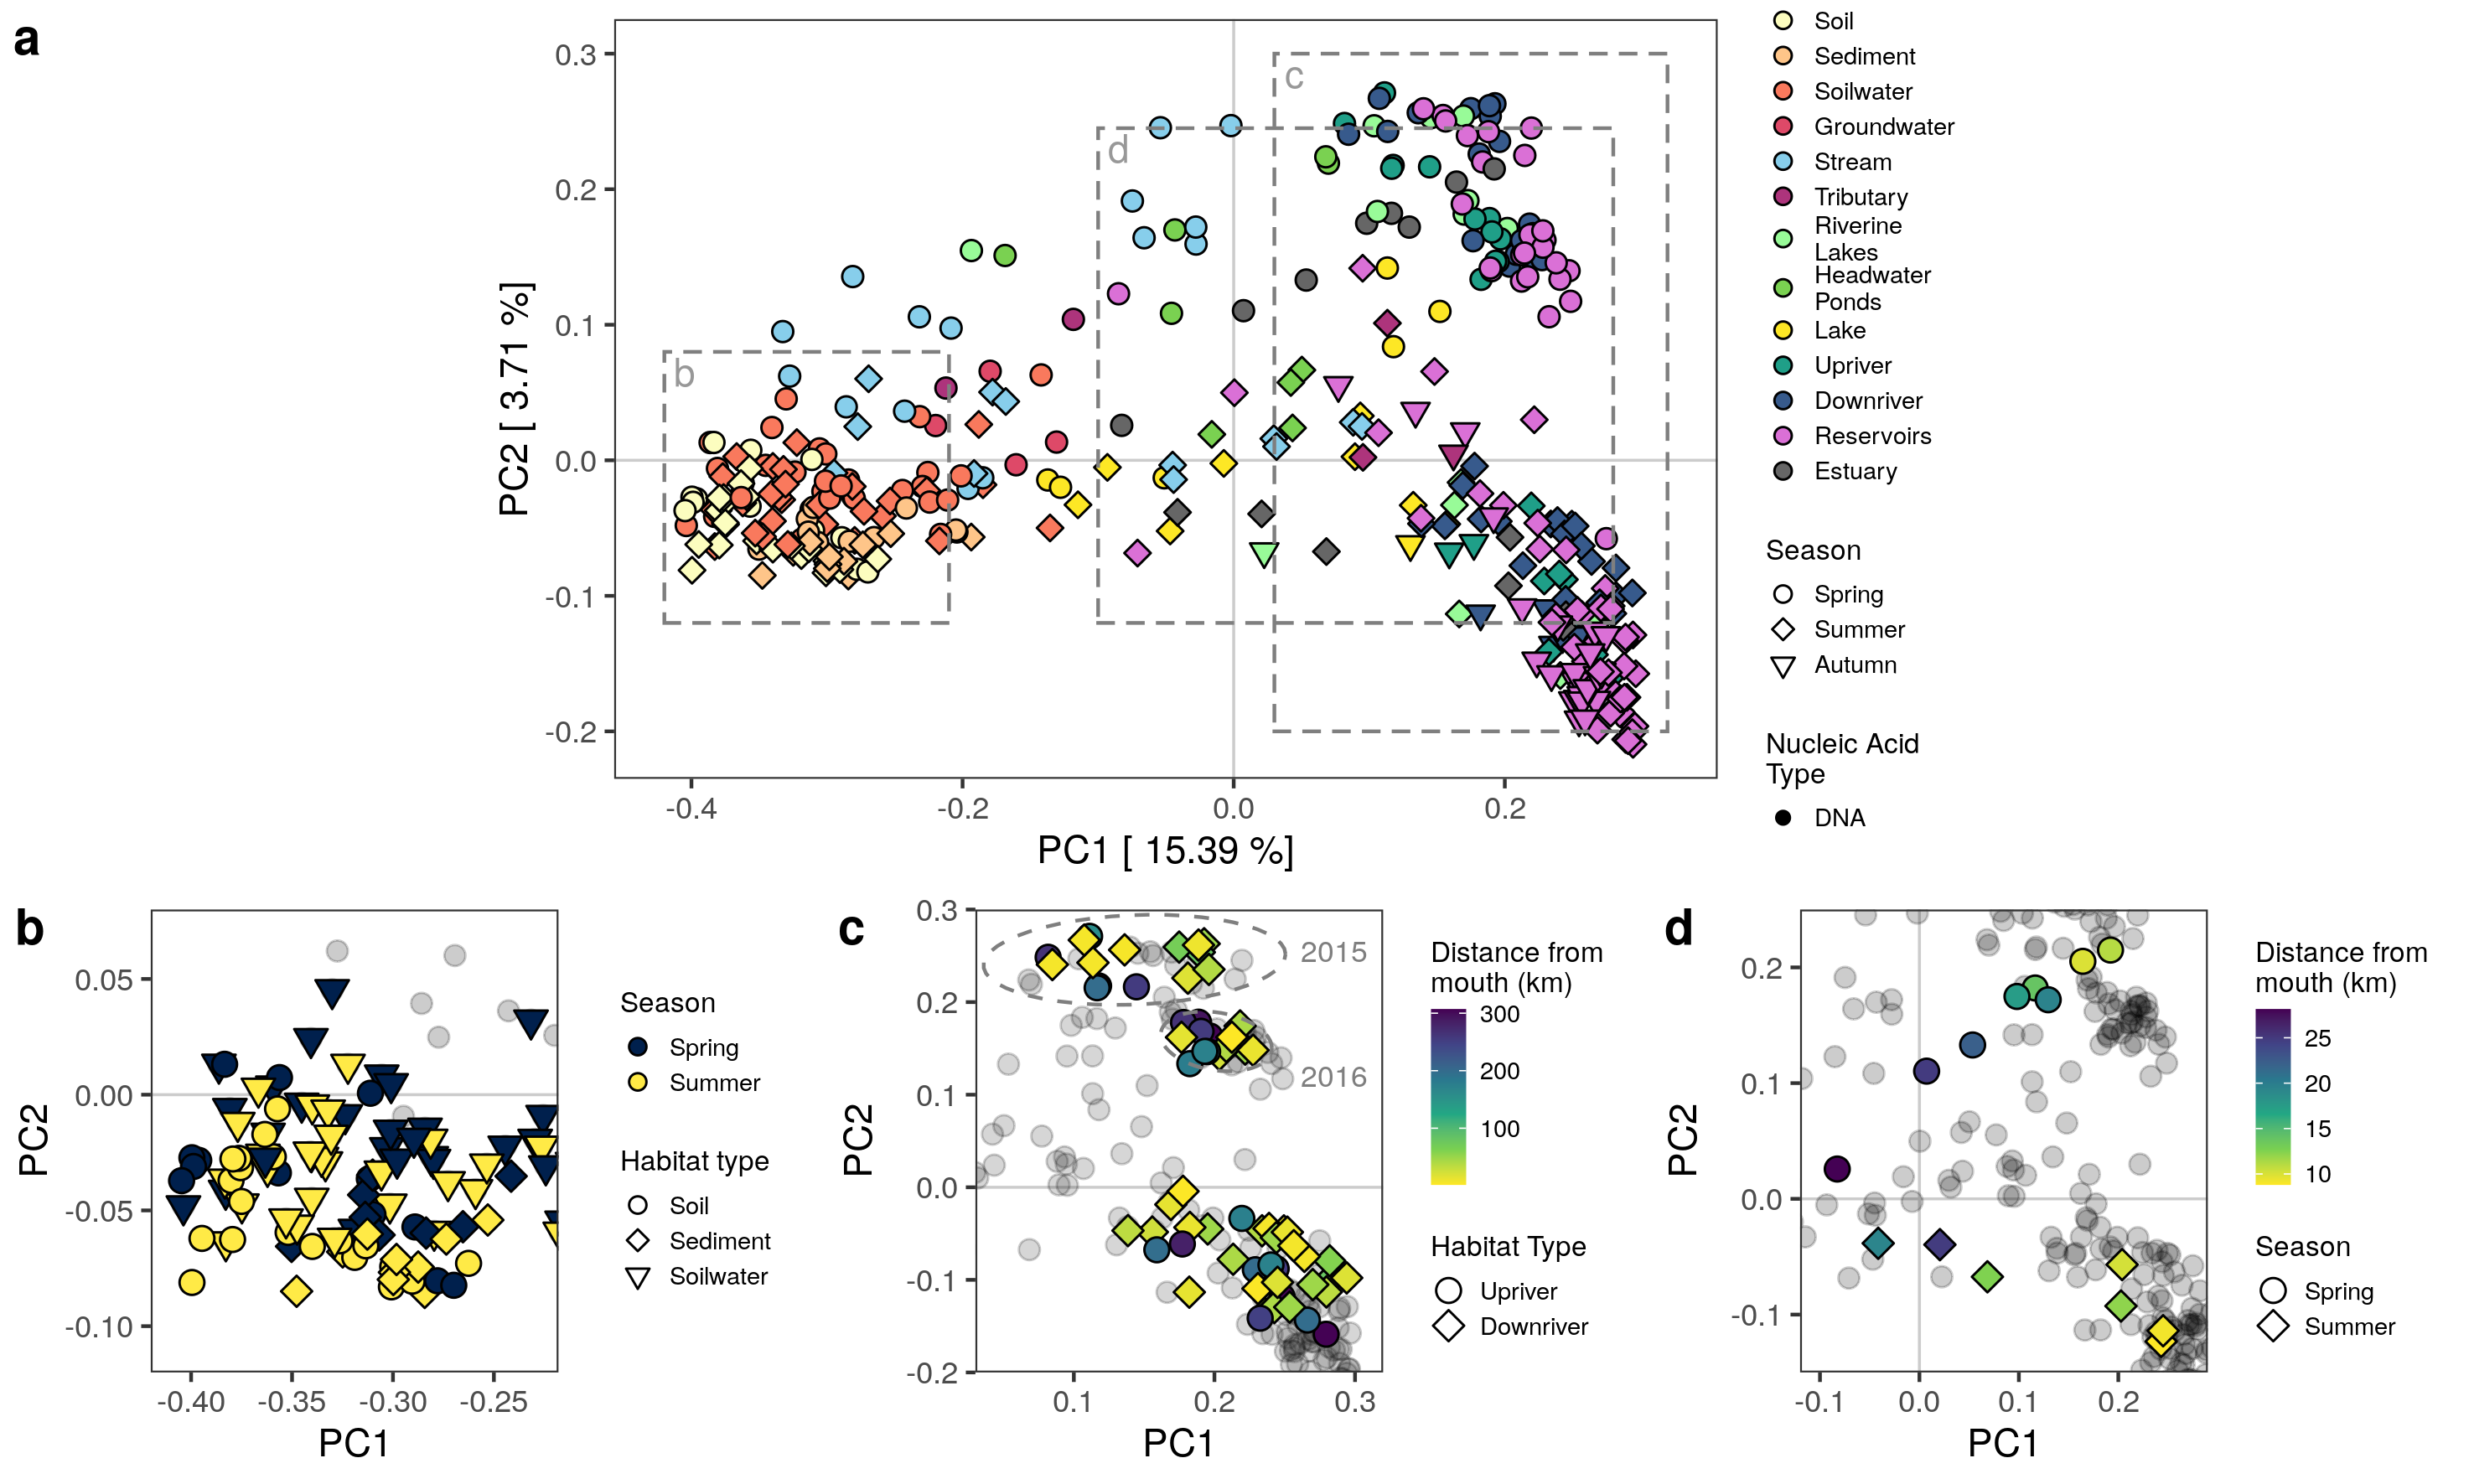
\includegraphics[width=16cm]{../../Figures/Final/PCoA_hellin_DNA_collage.png}
\caption{\textbf{Microbial community composition gradually changes along a terrestrial-hyrodlogical continuum and diverges between seasons.} Overall PCoA analysis of DNA samples (a) has been further explored with focus plots on terrestrial, riverine and estuary samples in panels b, c, d, respectively. Overall, the PCoA reveals microbial community shifts from terrestrial to freshwater samples. Spring and summer/autumn show distinct paths in multivariate space. Percentage of variance explained are given in square brackets for the first and second axes.}
%includegraphics[width=1\textwidth]
\end{figure}

\begin{figure}[!ht]
\centering
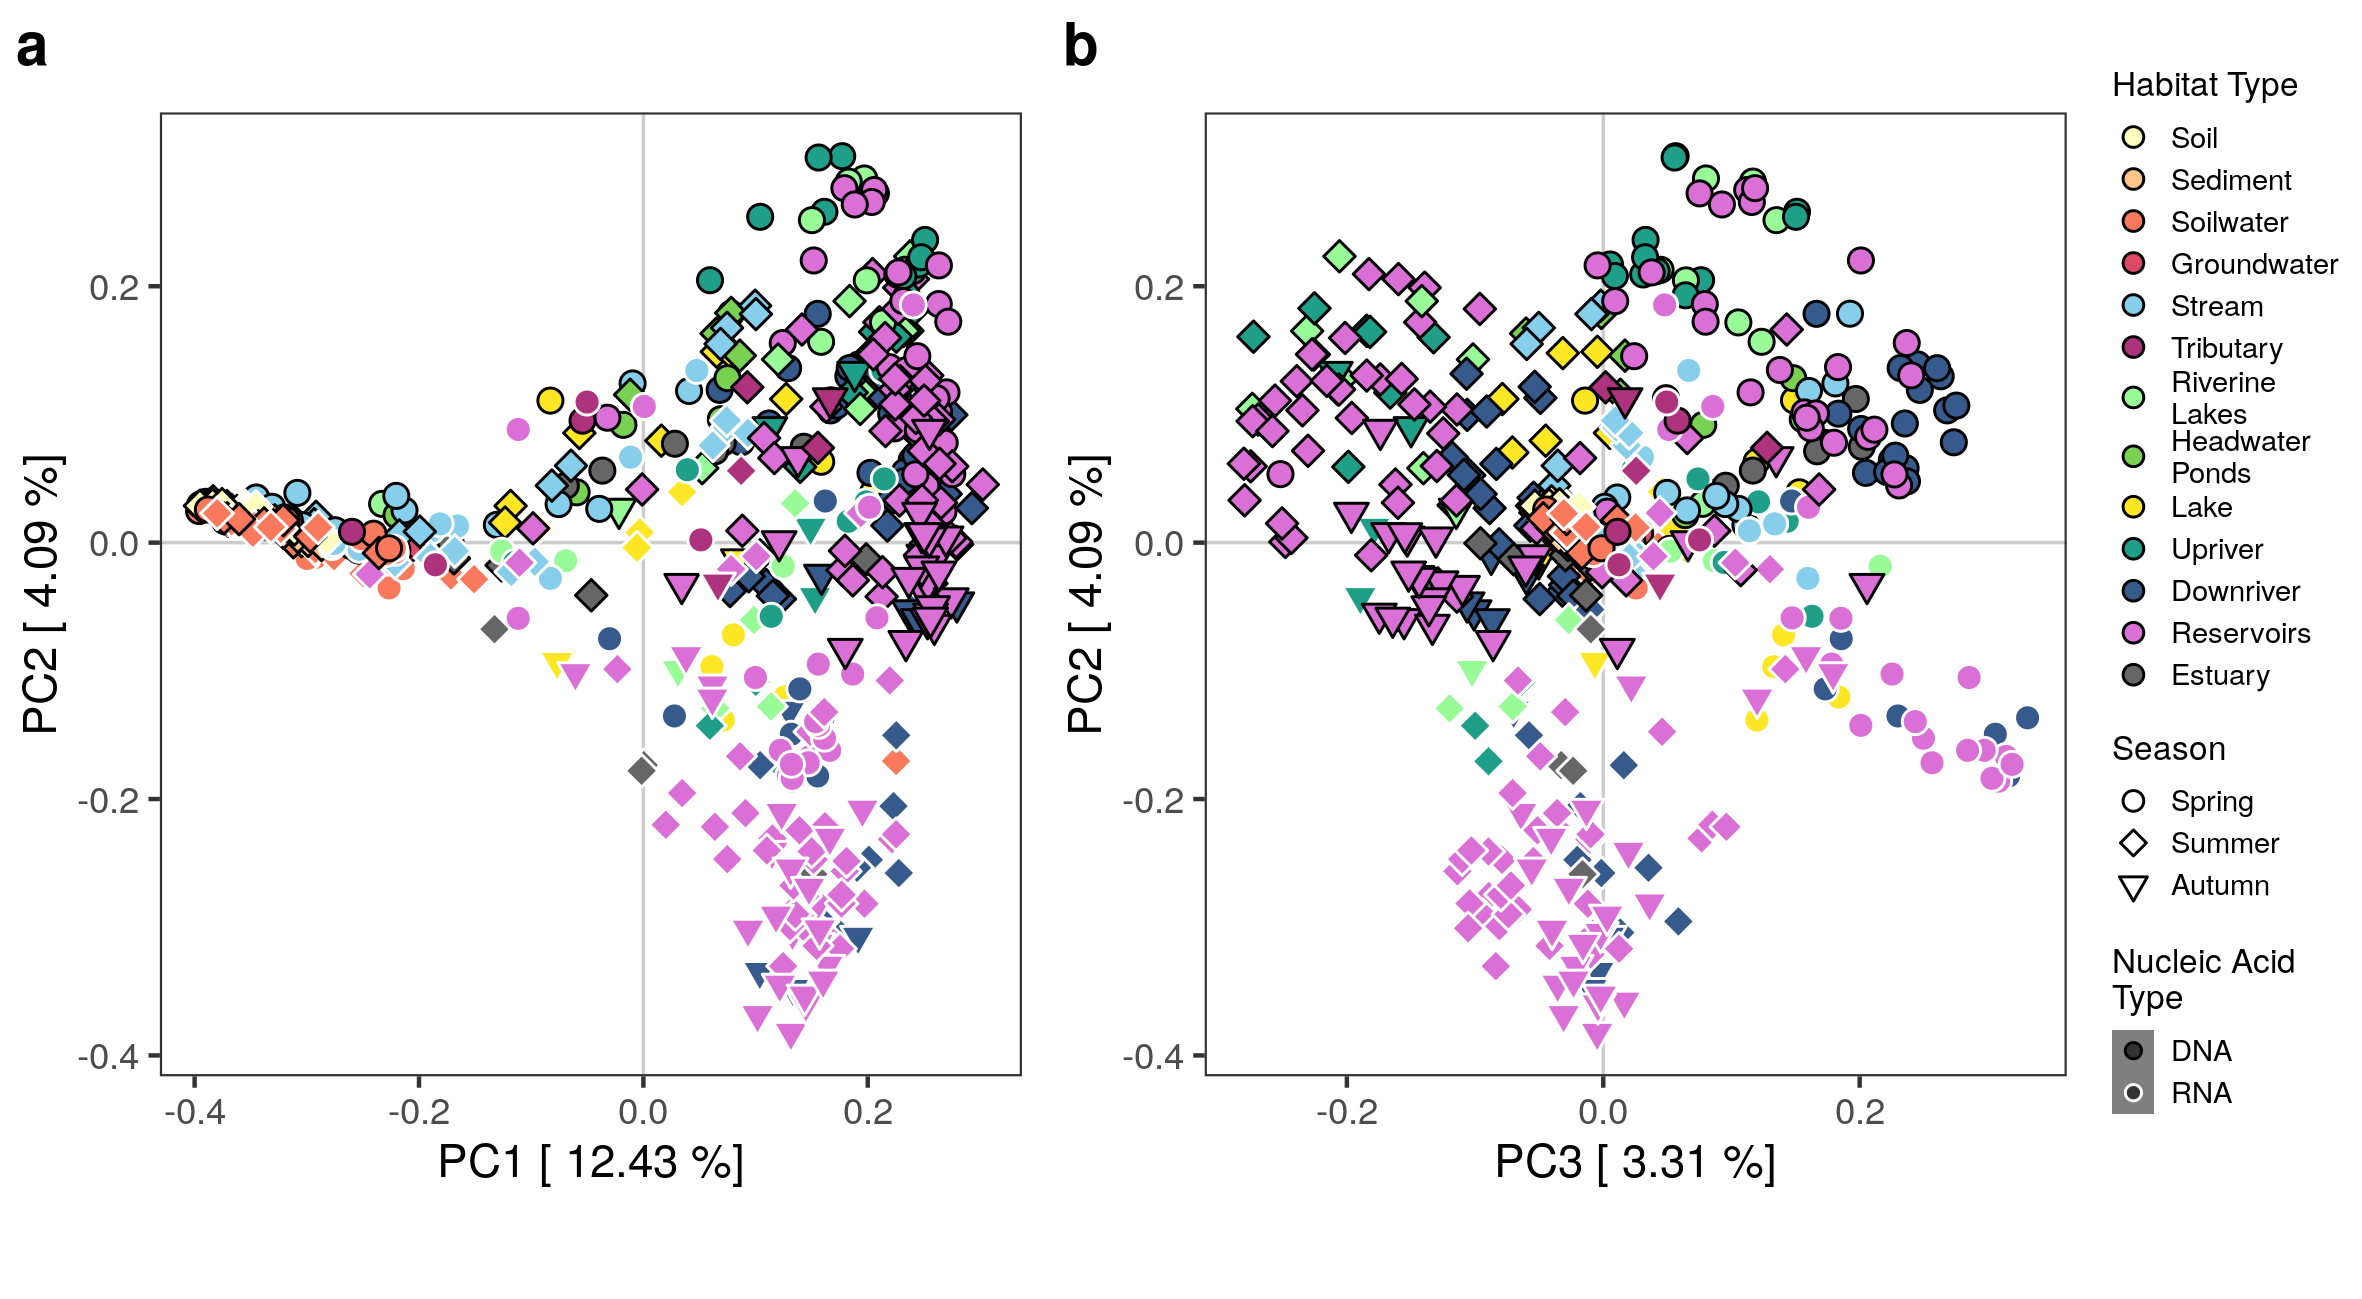
\includegraphics[width=17cm]{../../Figures/Final/PCoA_all_SampleType.png}
\caption{\textbf{RNA assemblages diverge from DNA within aquatic habitats, less so in terrestrially influenced habitats.} PCoA analysis including RNA samples. a) Visualization of first and second axes of PCoA, differentiating habitat type and nucleic acid type, respectively. b) Different view on PCoA analysis using the second and third axes, differentiating nucleic acid type and seasons, respectively. Percentage of variance explained by the corresponding axes are given in square brackets.}
%includegraphics[width=1\textwidth]
\end{figure}

\begin{figure}[!ht]
\centering
\includegraphics[width=15cm]{../../Figures/Final/distance_lollipop.png}
\caption{\textbf{Patterns between abundance and incidence-based distance reveal habitats dominated by selection and mass effects, respectively.} a) Distances between DNA and RNA of the same sample within ordination space were averaged by habitat type and season. Abundance based (coloured points, m\textsubscript{BC}) and incidence based distance (hollow points, m\textsubscript{S}) indicate spatio-seasonal trends of strong mass effects (high incidence distance) and selection (high abundance distance) along the terrestrial-aquatic continuum. b) $\Delta$ distances between m\textsubscript{BC} and m\textsubscript{S}. Patterns indicate shifts in the relative contribution of incidence vs. abundance based distances along the continuum, with increasing and decreasing trends corresponding to abundance and incidence driven dissimilarity, respectively. Habitats sampled outside the direct continuum give an additional meta-community context.}
%includegraphics[width=1\textwidth]
\end{figure}

\begin{figure}[!ht]
\centering
\includegraphics[width=15cm]{../../Figures/Final/first.observed.contribution.medianbins}
\caption{\textbf{Different taxa along the whole rank abundance curve contribute to the reactive pool.} a) Contribution of taxa (operational taxonomic units (OTUs)) detected in both DNA and RNA to the total number of RNA reads for each habitat type and season. OTUs were binned by 1) their first detected habitat in DNA along the continuum, 2) local DNA abundance (e.g. abundant, moderate, rare, see methods) and 3) whether they are above or below the overall median of all \% RNA contributions. Thus, values represent means of all OTUs falling in the same category. b) Proportion of DNA reads associated to taxa categorized by their first detected habitat in DNA and that fall above or below the \% RNA contribution median or OTUs without any RNA detection (RNA = 0). As observed in panel a) > Median and < Median OTUs are seemingly reactive and unreactive, respectively. Values are expressed as a fraction of the total number of DNA reads for each habitat type and season.}
%includegraphics[width=1\textwidth]
\end{figure}

\begin{figure}[!ht]
\centering
\includegraphics[width=15cm]{../../Figures/Final/spag_contribution}
\caption{\textbf{Taxa shifting between abundance groups contribute most prominently to the RNA pool.} a) Proportion of OTUs categorized by their DNA spatial abundance group (spAGs, see Tab.1) in each habitat where they were first detected in. b) Contribution of OTUs to the total RNA fraction of each habitat type and season. OTUs are categorized by spAGs, whether they are above or below the overall \% RNA contribution median and where they were first detected in. The middle line represents the median, lower and upper hinges of boxplots correspond to the 25th and 75th percentiles. Upper and lower whiskers expand to the largest and smallest value, respectively, but no further than 1.5 times the inter-quartile range from the hinge. Points beyond whiskers are represented as outlier points.}
%includegraphics[width=1\textwidth]
\end{figure}


\end{document}
